\documentclass{standalone}
\usepackage{pgfplots}
\usepackage{amsmath}
\usetikzlibrary{calc}
\pgfplotsset{compat=newest}
\pgfplotsset{every axis/.append style={line width=0.5pt}}
\tikzset{mark size=1.0}
\begin{document}
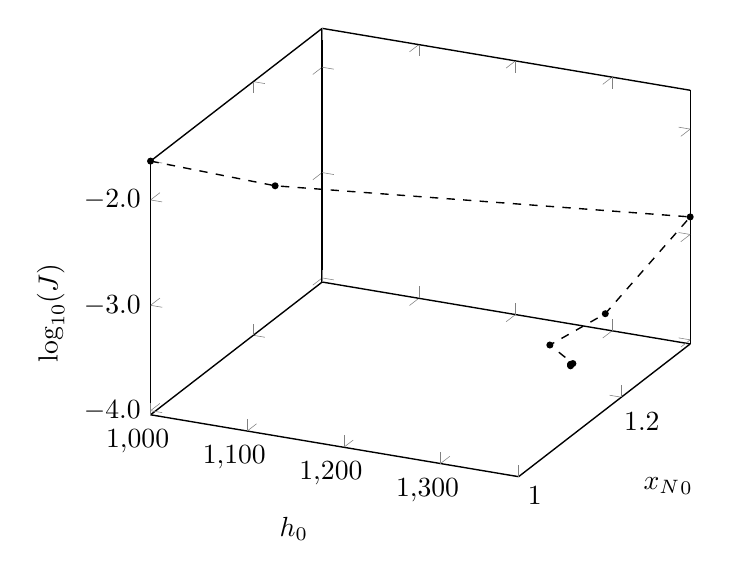
\begin{tikzpicture}
\begin{axis}[
scaled ticks=false,
enlargelimits=false,
% zmin = 0.0,
zticklabel style={
anchor=east,
/pgf/number format/precision=1,
/pgf/number format/fixed,
/pgf/number format/fixed zerofill,
},
xlabel=$h_0$, ylabel=${x_N}_0$, zlabel=$\text{log}_{10}(J)$,
]
\addplot3[dashed, mark=*, mark options=solid] table[x=h,y=phi,z=j] {
h phi j
1000.0 1.0 -1.63129322134
1100.0 1.05433705941 -1.91633995646
1380.82171628 1.33407141424 -2.83341463733
1324.20961183 1.27524478863 -3.61747665936
1288.17381783 1.23515088358 -3.8190864821
1303.14471288 1.25184643527 -4.03469745156
1301.8192207 1.2501486357 -4.03819246455
1301.82909919 1.24989590641 -4.03827054215
1302.09736321 1.24918517414 -4.03847555363
1303.16002089 1.24724350067 -4.03901077505
};
\end{axis}
\end{tikzpicture}
\end{document}